This appendix contains diagrams of the topologies to be tested, configured according to Section 3.2. The networks were visualized with CytoScape \cite{shannon_cytoscape_2003}. Unless specified, the topologies are from the Internet Topology Zoo. In all diagrams, Green nodes are servers, Purple nodes are clients, and Orange nodes are switches.
\begin{figure}
    \centering
    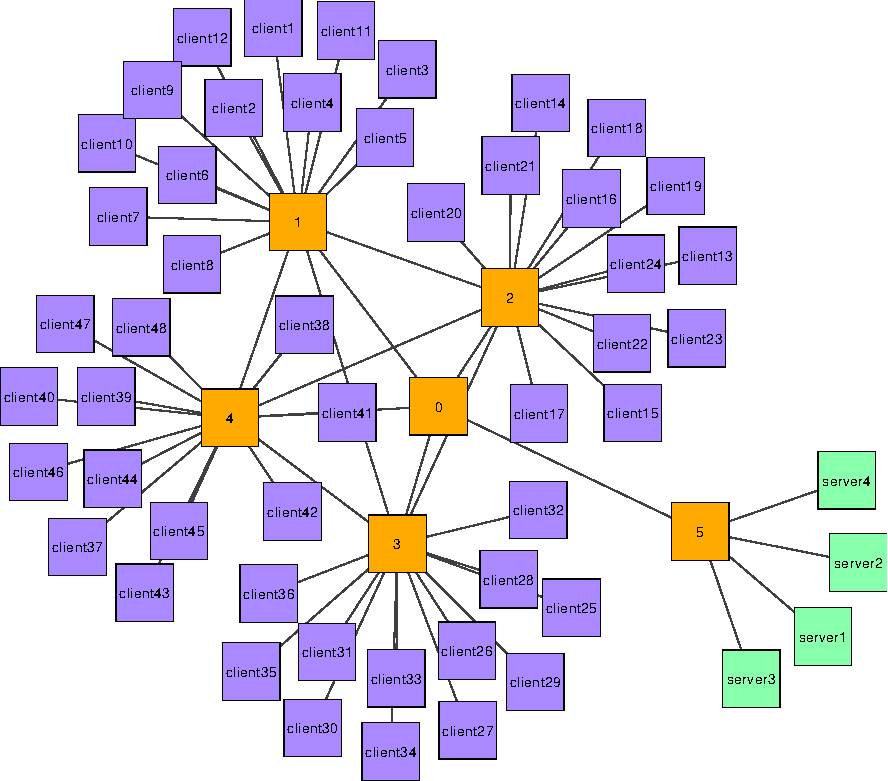
\includegraphics[width=\linewidth]{Networks/Complete Graph_final.pdf}
    \caption{Complete Mesh Topology with 5 nodes in the mesh}
    \label{fig:CompleteMesh}
\end{figure}

\begin{figure}
    \centering
    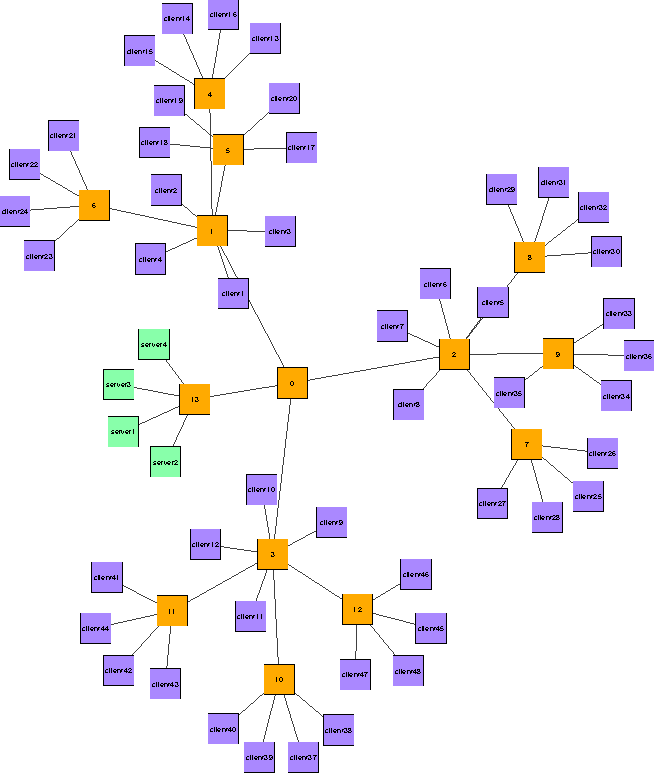
\includegraphics[width=\linewidth]{Networks/Balanced Tree_final.pdf}
    \caption{Fat-Tree Topology with fanout 3 and height 2}
    \label{fig:BalancedTree}
\end{figure}

\begin{figure}
    \centering
    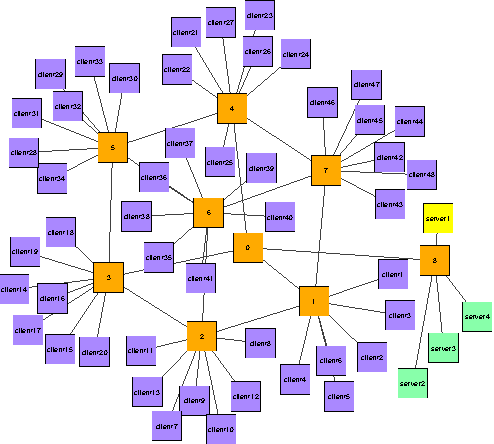
\includegraphics[width=\linewidth]{Networks/Hypercube_final.pdf}
    \caption{Hypercube Topology with 8 nodes and 12 edges}
    \label{fig:Hypercube}
\end{figure}

\begin{figure}[htbp]
    \centering
    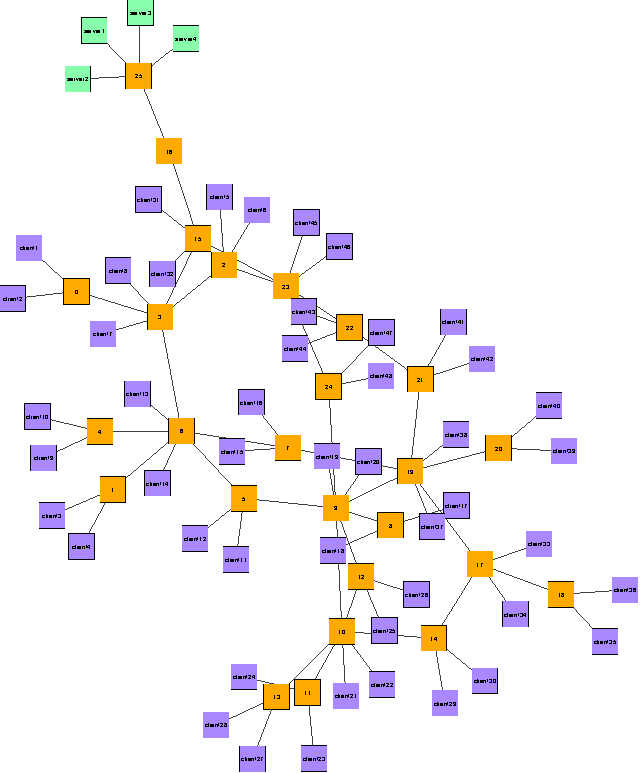
\includegraphics[width=\linewidth]{Networks/Agis_final.pdf}
    \caption{Agis Topology}
    \label{fig:Agis}
\end{figure}

\begin{figure}[htbp]
    \centering
    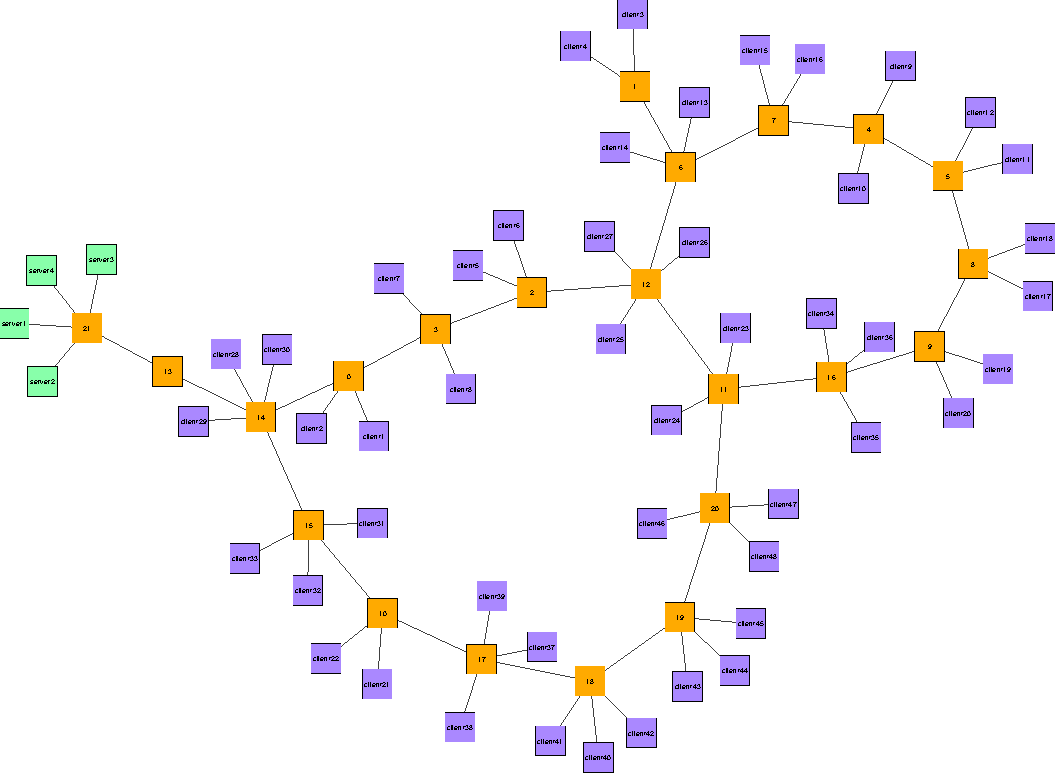
\includegraphics[width=\linewidth]{Networks/Atmnet_final.pdf}
    \caption{Atmnet Topology}
    \label{fig:Atmnet}
\end{figure}

\begin{figure}[htbp]
    \centering
    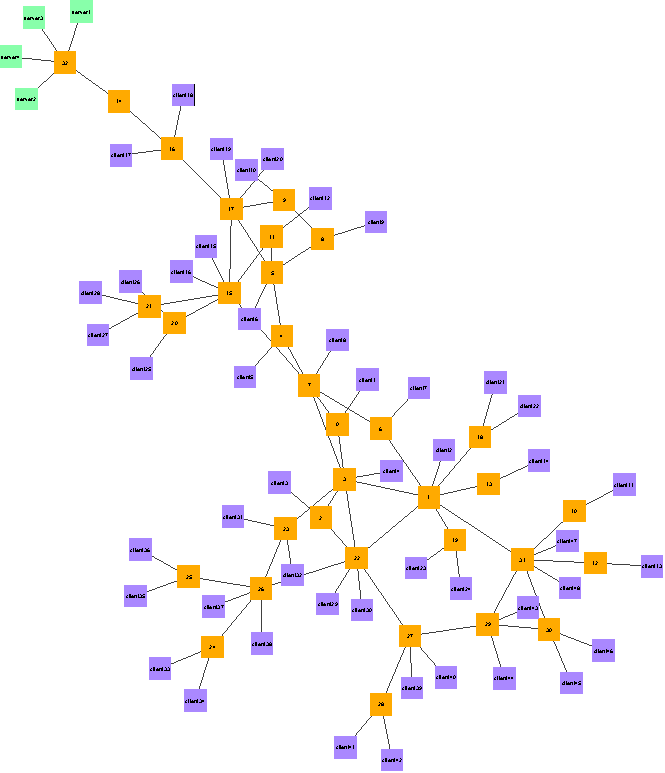
\includegraphics[width=\linewidth]{Networks/Canerie_final.pdf}
    \caption{Canerie Topology}
    \label{fig:Canerie}
\end{figure}

\begin{figure}[htbp]
    \centering
    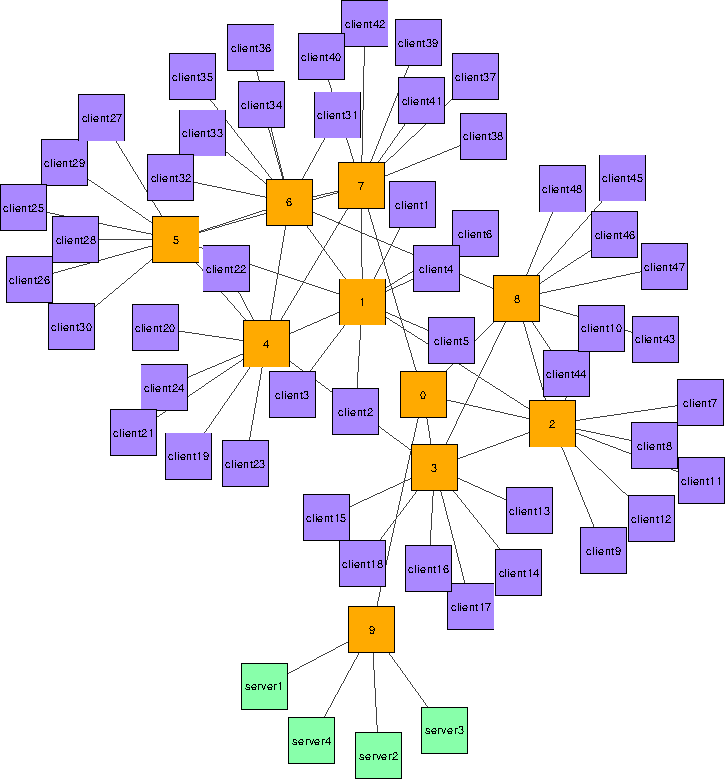
\includegraphics[width=\linewidth]{Networks/Gridnet_final.pdf}
    \caption{Gridnet Topology}
    \label{fig:Gridnet}
\end{figure}

\begin{figure}[htbp]
    \centering
    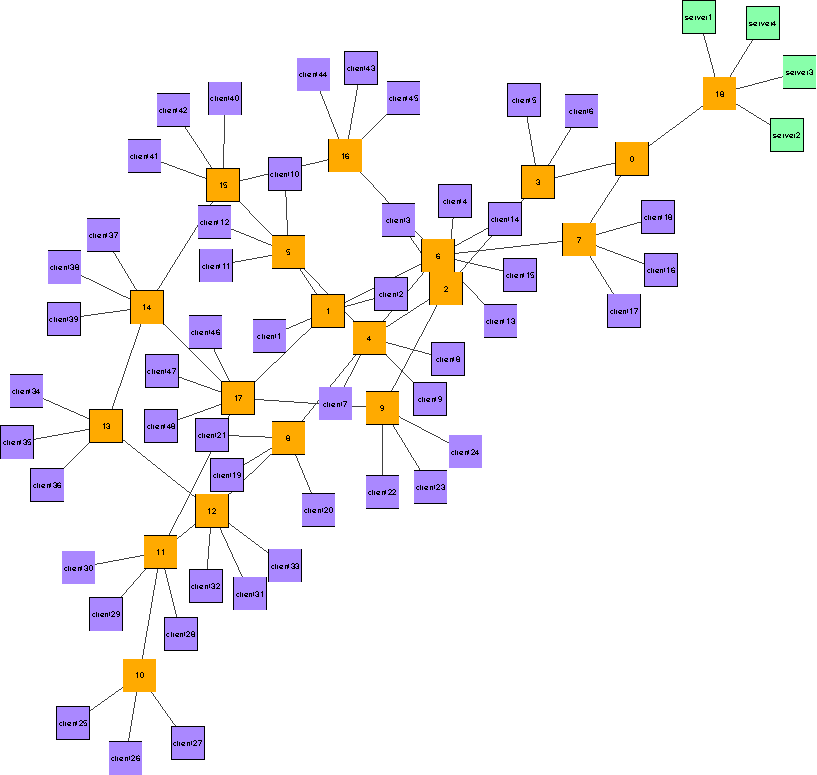
\includegraphics[width=\linewidth]{Networks/Ibm_final.pdf}
    \caption{Ibm Topology}
    \label{fig:Ibm}
\end{figure}

\begin{figure}[htbp]
    \centering
    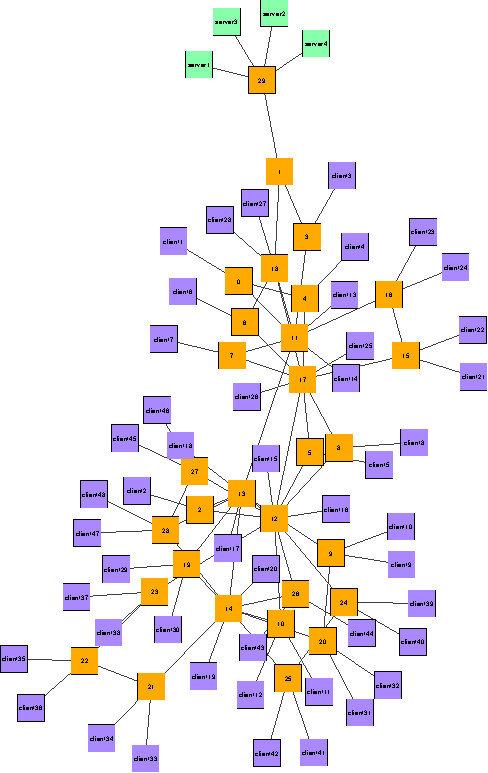
\includegraphics[width=\linewidth, height=\textheight]{Networks/Janetbackbone_final.pdf}
    \caption{Janetbackbone Topology}
    \label{fig:Janetbackbone}
\end{figure}

\begin{figure}[htbp]
    \centering
    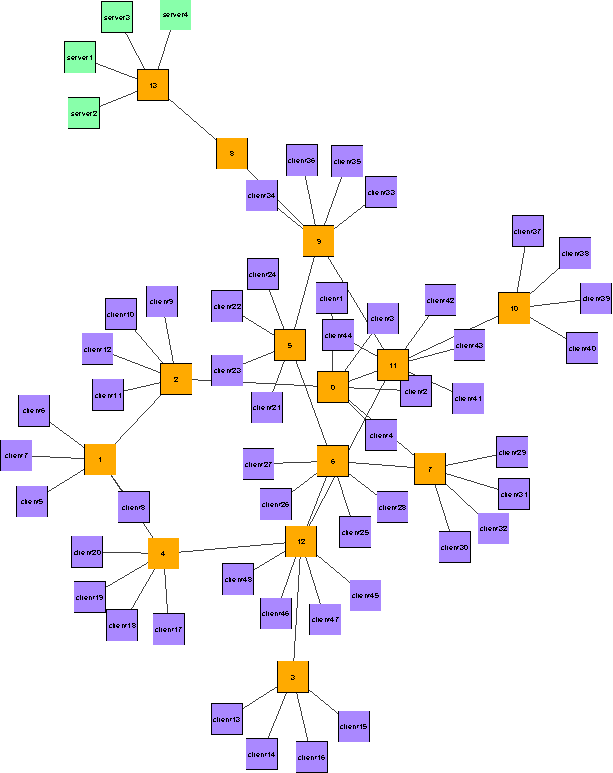
\includegraphics[width=\linewidth]{Networks/Nsfnet_final.pdf}
    \caption{Nsfnet Topology}
    \label{fig:Nsfnet}
\end{figure}

\begin{figure}[htbp]
    \centering
    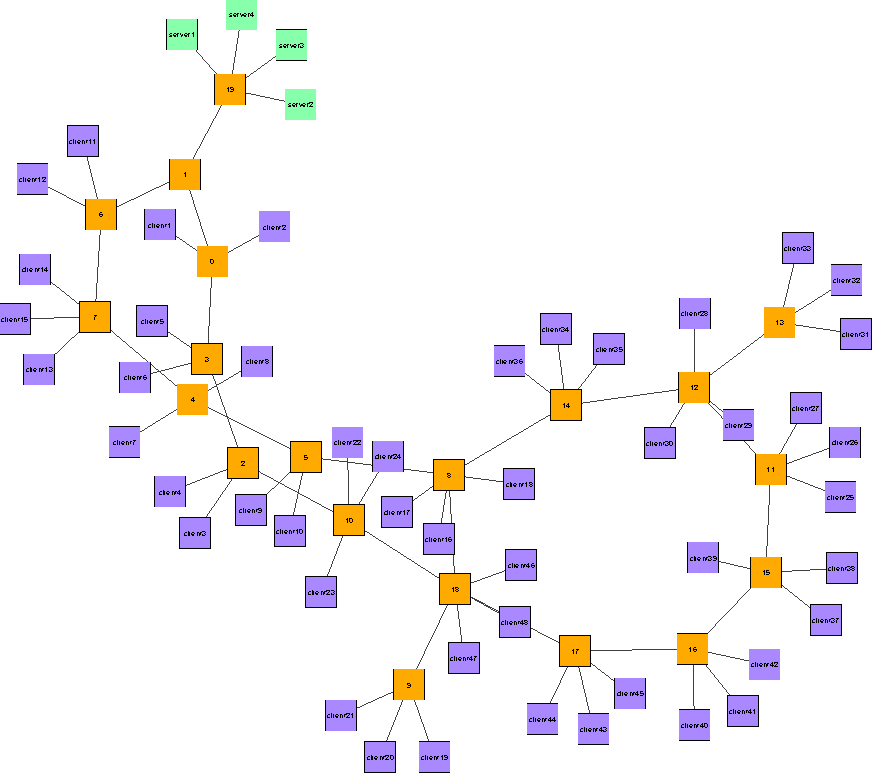
\includegraphics[width=\linewidth]{Networks/Savvis_final.pdf}
    \caption{Savvis Topology}
    \label{fig:Saavis}
\end{figure}

\begin{figure}[htbp]
    \centering
    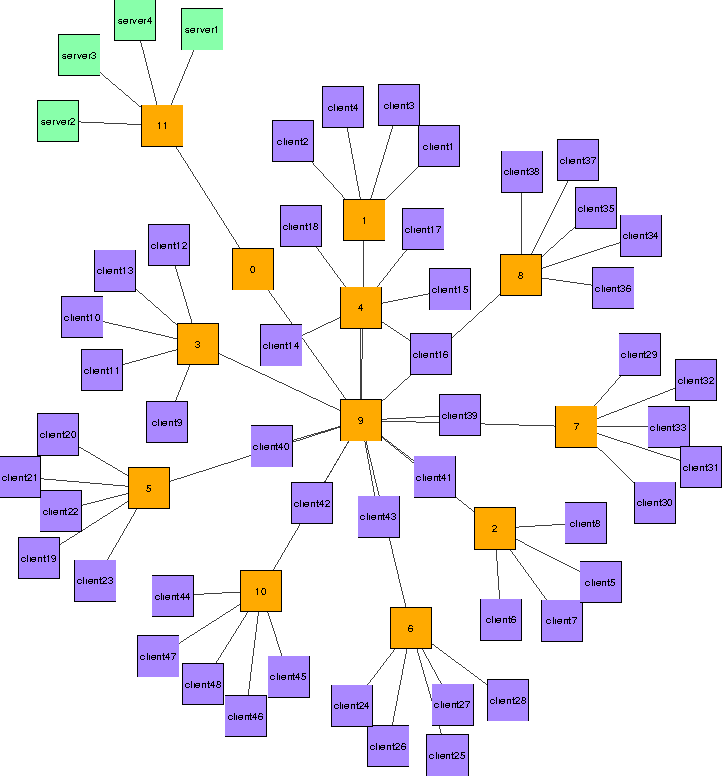
\includegraphics[width=\linewidth]{Networks/Singaren_final.pdf}
    \caption{Singaren Topology}
    \label{fig:Singaren}
\end{figure}

\begin{figure}[htbp]
    \centering
    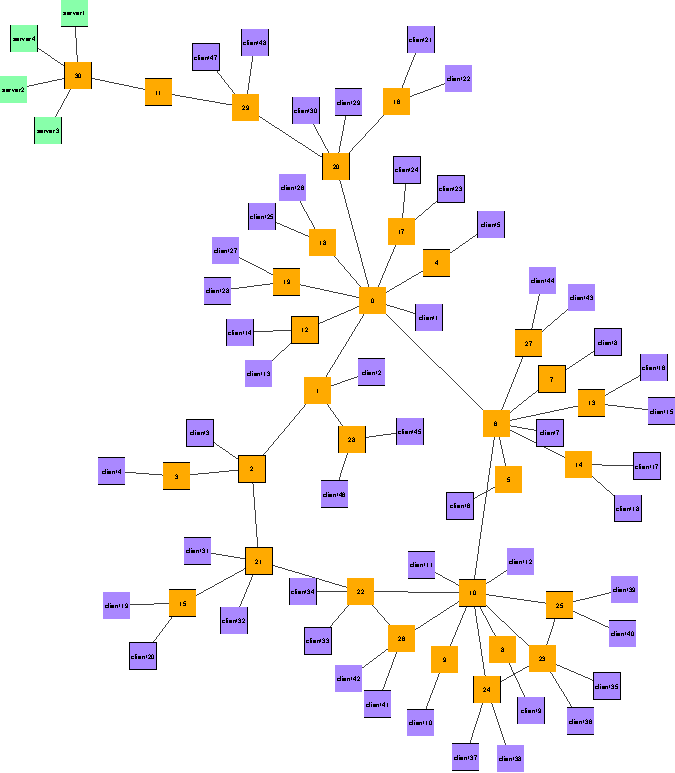
\includegraphics[width=\linewidth]{Networks/WideJpn_final.pdf}
    \caption{WideJpn Topology}
    \label{fig:WideJpn}
\end{figure}